\section{Random Sampling}


\begin{center}
	\begin{figure}[H]
		\subfloat[Fossil]{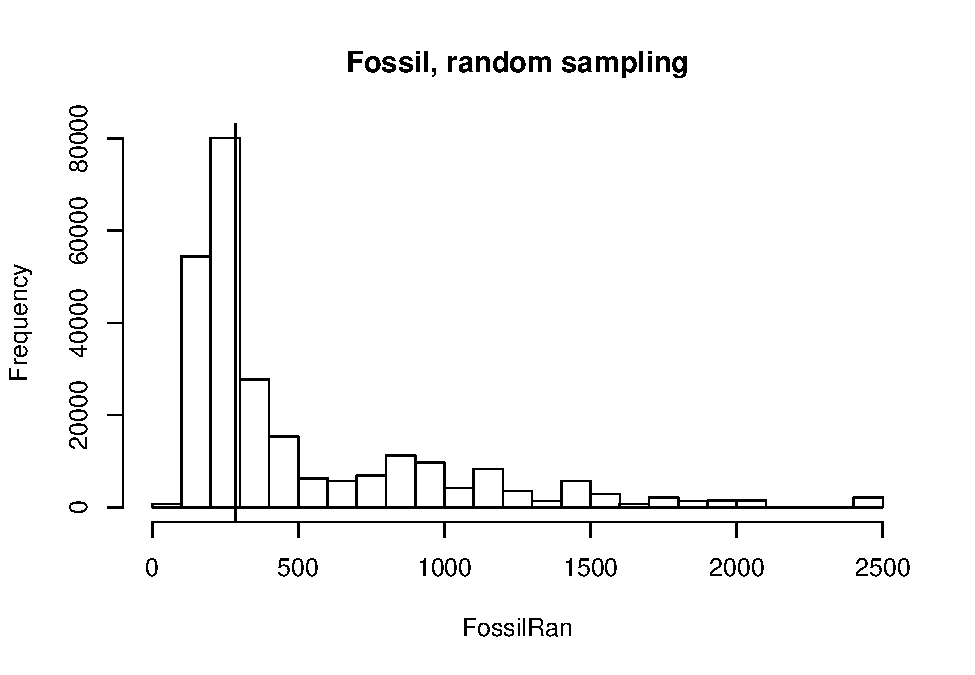
\includegraphics[scale=0.45]{MA_JJ_files/figure-latex/RSFM-1.pdf}}
		\subfloat[Modern, insular]{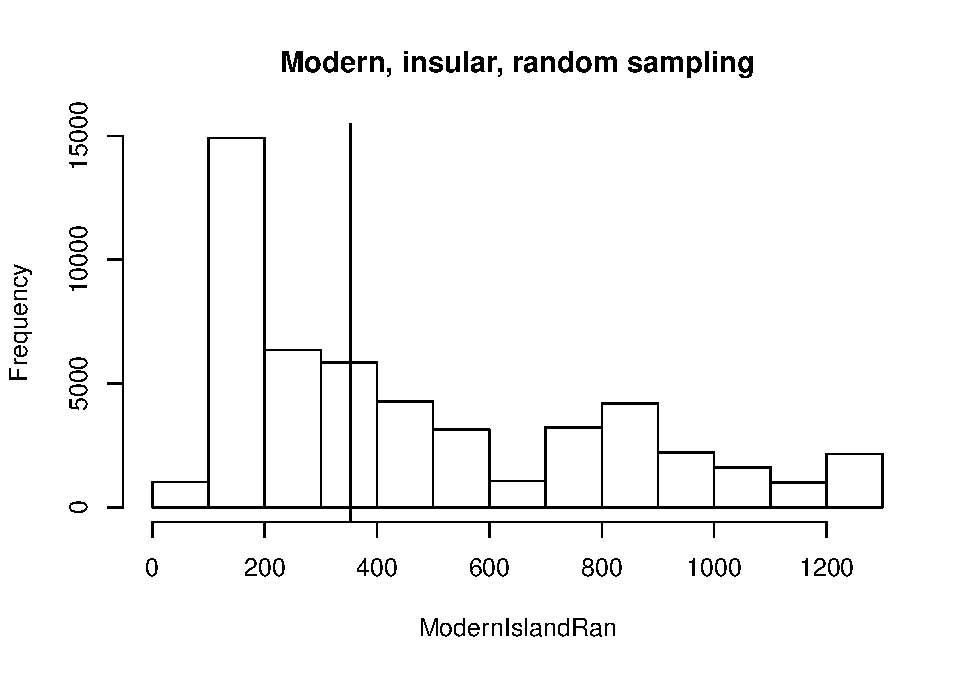
\includegraphics[scale=0.45]{MA_JJ_files/figure-latex/RSMFCI-1.pdf}}	
		\hfill %
		\subfloat[Fossil, continental]{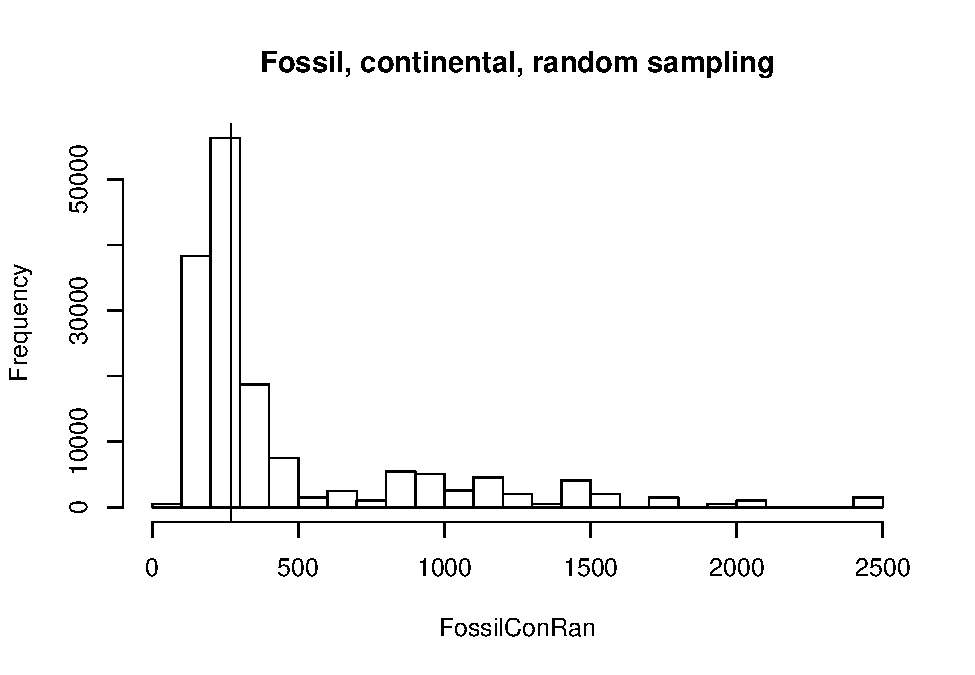
\includegraphics[scale=0.45]{MA_JJ_files/figure-latex/RSMFCI-2.pdf}}
		\subfloat[Continental]{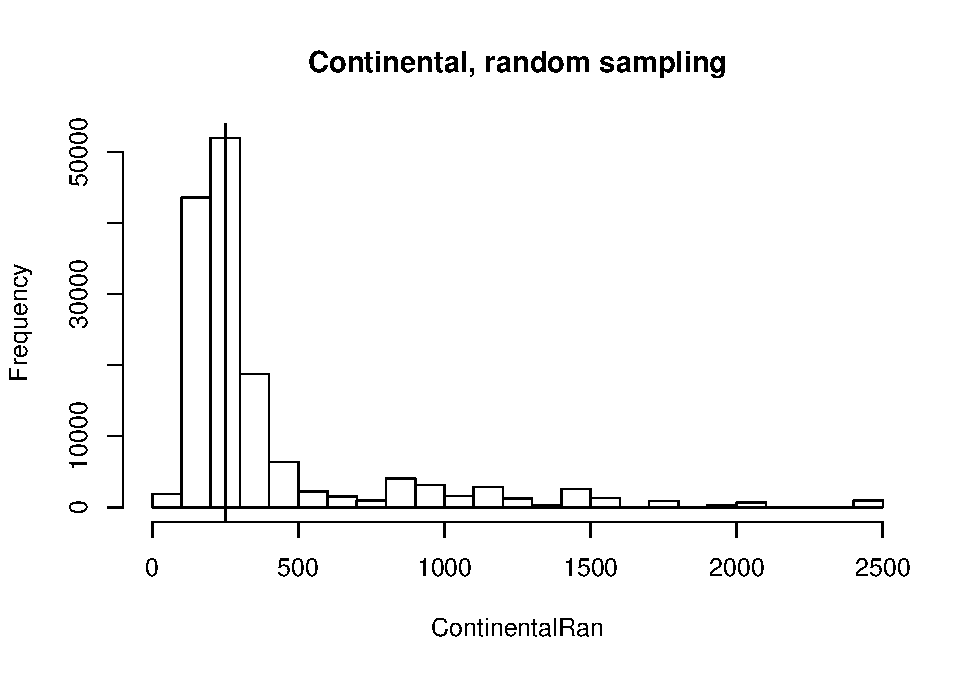
\includegraphics[scale=0.45]{MA_JJ_files/figure-latex/RSCI-1.pdf}}
		\caption[Random sampling]{Random sampling for several subgroups. For (a), (c), and (d) the random sample reflects the real sample, for (b) this is not the case.}
		\label{fig:RSadd}
	\end{figure}
\end{center}



\begin{center}
	\begin{figure}[H]
		\subfloat[America]{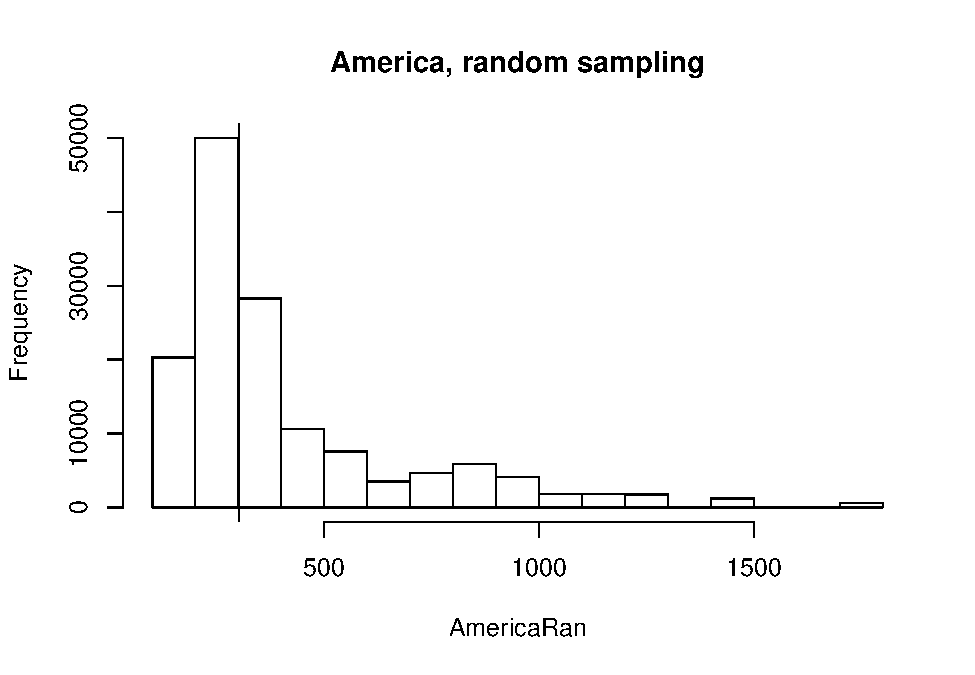
\includegraphics[scale=0.3]{MA_JJ_files/figure-latex/RSCon-1.pdf}}
		\subfloat[Europe]{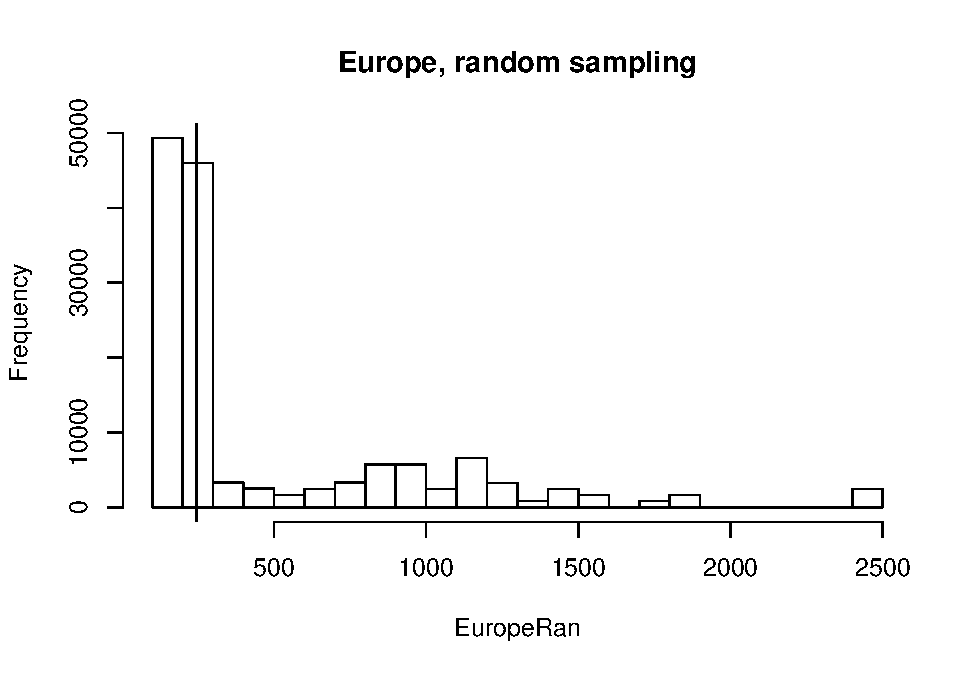
\includegraphics[scale=0.3]{MA_JJ_files/figure-latex/RSCon-2.pdf}}	
		\subfloat[Eurasia]{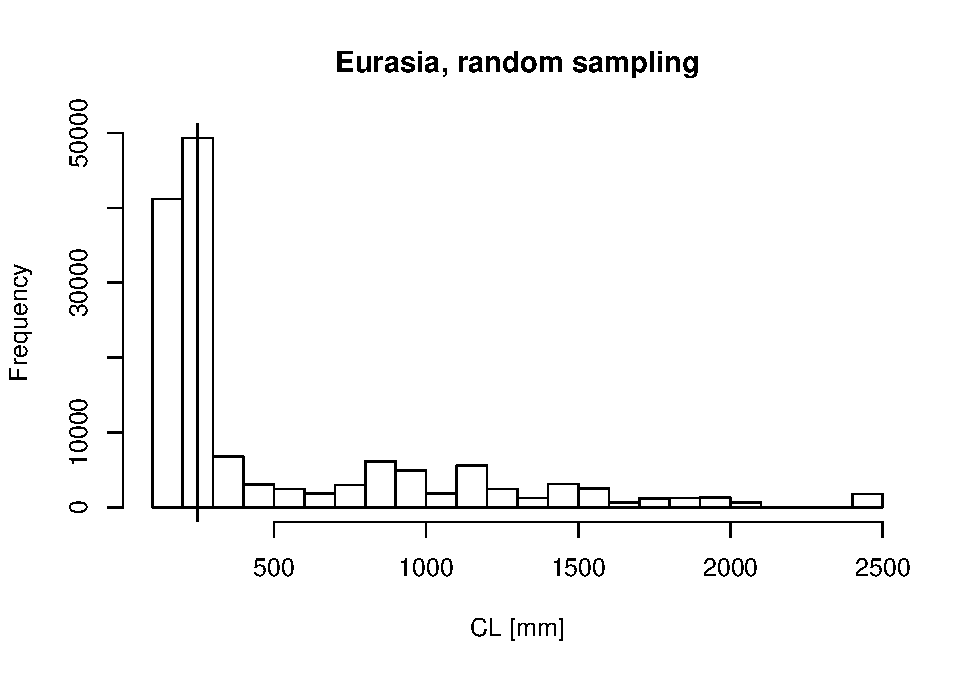
\includegraphics[scale=0.3]{MA_JJ_files/figure-latex/RSCon-3.pdf}}
		\caption[Random sampling, continents]{Random sampling for different continents. All random samples reflect the real sample.}
		\label{fig:RSadd}
	\end{figure}
\end{center}

